\documentclass{standalone}
\usepackage{diplomski}

\begin{document}

\chapter{Laboratory setup} \label{ch:setup}
\pagenumbering{arabic}
\setcounter{page}\thestranica

% --------------------------------------

The implemented system is a distributed fibre-optical sensor, built to be accessed only from the one side. In order to use Raman scattering for temperature measurement, a laser source must be capable of producing sufficiently short optical impulses, so as to meet spatial resolution requirements, as described by equation \ref{eq:otdr_resolution}. In this laboratory setup, an Optilab NPL-1550-37-R nanosecond pulse laser was used as the optical source. The laser is capable of producing pulses down to 2 ns in width, with a repetition rate of 100 Hz to 1 MHz \cite{datasheet:laser}. The energy of a single pulse can be up to 100 \textmu J. High optical power is achieved using an integrated dual-stage erbium-doped fibre amplifier (abbr. EDFA), capable of producing continuous optical power of 37 dBm, while operating in the 1543 -- 1570 nm region. High-power laser output is factory-coupled into a single-mode fibre pigtail. Also, a 1\% tap FC output is available, which will be used in this setup to trigger the DAQ device. This signal will also be used to measure peak optical power. \\

The measurement setup is displayed in Figure \ref{fig:lab_setup}.
\begin{figure}[b]
	\centering
	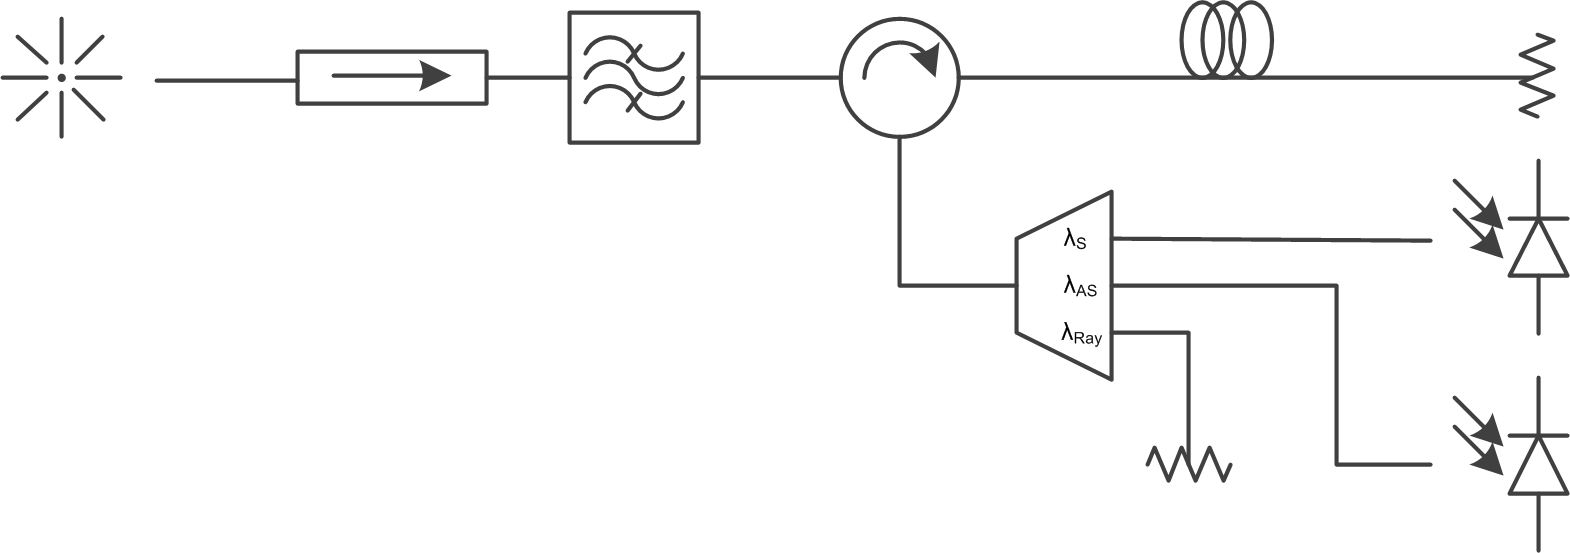
\includegraphics[width=\textwidth]{lab_setup.png}
	\caption{Block diagram of a Raman reflectometer}
	\label{fig:lab_setup}
\end{figure}
The laser's high-power output is protected from backscattered signals by an isolator placed immediately after the output pigtail. Although the majority of amplified spontaneous emission (abbr. ASE) from laser's integrated amplifiers is already filtered, an additional filter is placed after the isolator, to ensure maximum noise suppression. The selected filter is a dense wavelength-division multiplex (abbr. DWDM) filter, centred at
\begin{equation} \label{eq:dwdm_filter_centre}
\lambda_0 = \SI{1550}{\nano \meter}
\end{equation} and pass bandwidth 
\begin{equation} \label{eq:dwdm_filter_bw}
\varDelta f = \SI{200}{\giga \hertz} \textrm{.}
\end{equation}
Although the filter is specified to be able to withstand a continuous optical power of 500 mW, the expected tolerance to peak power in pulse regime is much higher. Connecting the rest of the measurement setup to filter's \textit{pass} output, the initial ASE is now ensured to be negligible. \\

The circulator placed after the DWDM filter is an important component in the measurement setup. In the first setup, single-mode fibres were used as temperature sensing elements. Fibres coupled onto the circulator need to match the structure of the measurement fibre, so as to ensure good coupling and minimum losses of the pump signal and reflected signals. The circulator itself is a low insertion loss device and provides high isolation between ports. The circulator has single-mode pigtails. Its port 1 is coupled to the high-power output from the DWDM filter, port 2 to the measurement fibre, and port 3 to the monitoring branch of the system. \\

Measurement fibres can be single fibre-rolls, or consist of a cascade of fibre-rolls. In the single-mode setup, regular SM fibres, compliant with the ITU G.652 standard, were interchanged with highly non-linear fibres. The observed measurement fibre system had a total length of about 5 km. Parts of this fibre system can be inserted into a cooling or heating chamber in order to control the system temperature. The far end of the measurement fibre has to be terminated to reduce reflection of the incident high-power signal off the fibre end. Such a reflection could induce SRS, even powers that are normally expected to be sufficiently low to keep the system in spontaneous Raman-scattering regime. To achieve this, the one option is to use proper terminators. However, reflections can occur on unsuitable optical connectors, such as FC, that inherently exhibit high reflections. The other option is to couple the optical power into the environment, and ensure power containment by external means. \\

The latter solution was used in the second scenario, where multi-mode fibres replaced single-mode as sensing elements. Between the DWDM filter and the circulator, full optical power from single-mode-coupled laser was then coupled into multi-mode fibres. A single-mode circulator was replaced by a multi-mode version. The new circulator has multi-mode fibres factory-spliced onto its ports. It also exhibits low insertion losses, and high isolation. The high-power input is coupled to circulator's port 1, and the fibre-under-test is directly coupled onto port 2. Port 3 was also coupled to the monitoring branch. In the multi-mode scenario, the measurement fibre was expected to be able to withstand higher incident powers before exhibiting stimulated non-linear effects. The power threshold for SRS, from expression \ref{eq:raman_threshold}, is lowered, as a result of lower power density in the fibre. Therefore, a standard ITU G.651-compliant fibre was used for this purpose. A number of fibre rolls were spliced together to increase the total system length. Also, a short patch cable, 50 m in length, was inserted between two longer rolls. This simplified temperature control at a known point in the system. The patch was placed in a pot, in which heating and cooling of the fibre was performed by controlling the temperature of the water surrounding it. The isolation of the fibre patch was left unstripped to pertain its thermal and mechanical endurance. \\

The monitoring branch is connected to the circulator, so that the scattered signal from the measurement fibre is coupled into it. Three backscattered components need to be demultiplexed to monitor each component separately. A Raman wavelength-division multiplexer, the so-called \textit{Raman cube}, was used to achieve this. The two versions, one for the single-mode scenario, and the other for the multi-mode scenario, have one common port and three other ports centred at different wavelengths. One port is used to monitor Rayleigh scattering, one to monitor Stokes, and the third for anti-Stokes component. Central wavelengths for the three ports are
\begin{equation}
\lambda_\textrm{Ray} = \SI{1551}{\nano \meter}
\end{equation}
\begin{equation}
\lambda_\textrm{S} = \SI{1650}{\nano \meter}
\end{equation}
\begin{equation}
\lambda_\textrm{AS} = \SI{1450}{\nano \meter} \textrm{,}
\end{equation}
respectively. Some papers report the possibility of measurements of Raman-scattered components being biased due to the leakage of Rayleigh-scattered component through the Raman cube \cite{rayleigh_leakage1}\cite{rayleigh_leakage2}. The Raman cube used in this thesis has the isolation of critical couplings larger than 60 dB, which is sufficient to reduce cross-talk effects. \\

The Raman cube enables wavelength-demultiplexed scattered signals to be coupled into photodetectors. Three different InGaAs-based detectors by Thorlabs were tested here. Their optical and electrical characteristics are given in Table \ref{table:photodetectors} \cite{datasheet:pda10cf}\cite{datasheet:pda10cs}\cite{datasheet:apd130c}.
\begin{table}[t]
	\centering
	\caption{Optical and electrical characteristics of photodetectors}
	\label{table:photodetectors}
	\hspace*{-2em}
	\begin{tabular}{c|c|C{2cm}|C{2cm}|C{2cm}|C{2cm}|C{2cm}}
		\textbf{Model}	& \textbf{Type}	& \textbf{R [A/W] @ 1550$\,$nm}	& \textbf{Adjustable gain$\,$setting [dB]}	& \textbf{Transimp. gain [$\bm{\times 10^4 \textrm{V/A}}$]}	& \textbf{Bandwidth [MHz]}	& \textbf{NEP [$\bm{\textrm{pW}/\sqrt{\textrm{Hz}}}$]} \\ \hline \hline 
		PDA10CF-EC	& PIN	& 1.02	& --	& 1	& 150	& 12.0 \\ \hline
		\multirow{3}{*}{PDA10CS-EC}	& \multirow{3}{*}{PIN}	& \multirow{3}{*}{1.05}	& 20	& 1.5	& 1.9	& 3.0 \\ 
		& & & 30	& 4.75	& 0.775	& 1.25 \\
		& & & 40	& 15.1	& 0.320	& 1.40 \\ \hline
		APD130C	& APD	& 9	& --	& 10	& 50	& 0.46 \\
	\end{tabular}
\end{table}
For the PIN diode with switchable gain, the gain-bandwidth product is
\begin{equation}
\textrm{GBP} = \SI{600}{\mega \hertz} \textrm{.}
\end{equation}
Although these detectors are able to provide large gains, which are needed to monitor signals as weak as Stokes and anti-Stokes backscatterings, integrated amplifiers will not be able to provide sufficient bandwidth to faithfully detect the waveform of these signals. For the APD diode, the multiplication factor is
\begin{equation}
\textrm{M} = 10 \textrm{.}
\end{equation}
Although APD diodes normally exhibit larger noise in comparison to PIN diodes, this particular model provides very low noise powers, as well as inherent high gain and very large bandwidth. Therefore, in the final stage of this project, APD diode was installed to detect the anti-Stokes signal, as this signal has proven critical due to its low amplitude and high temperature dependence. The manufacturer of the APD photodiode indicated possible problems that may occur, as the detector size is only 0.2 mm in diameter. The light from the fibre tip is expected to diverge, leading to high coupling losses, especially in multi-mode applications. Some adaptations to the stock photodetector had to be made. An additional fibre collimator, aspheric focusing lens, as well as mechanical mounting devices were obtained from Thorlabs to ensure maximum light-coupling from the fibre to the photodetector. Schematic view of the optical setup at the photodetector is presented in Figure \ref{fig:apd_optics}.
\begin{figure}[h]
	\centering
	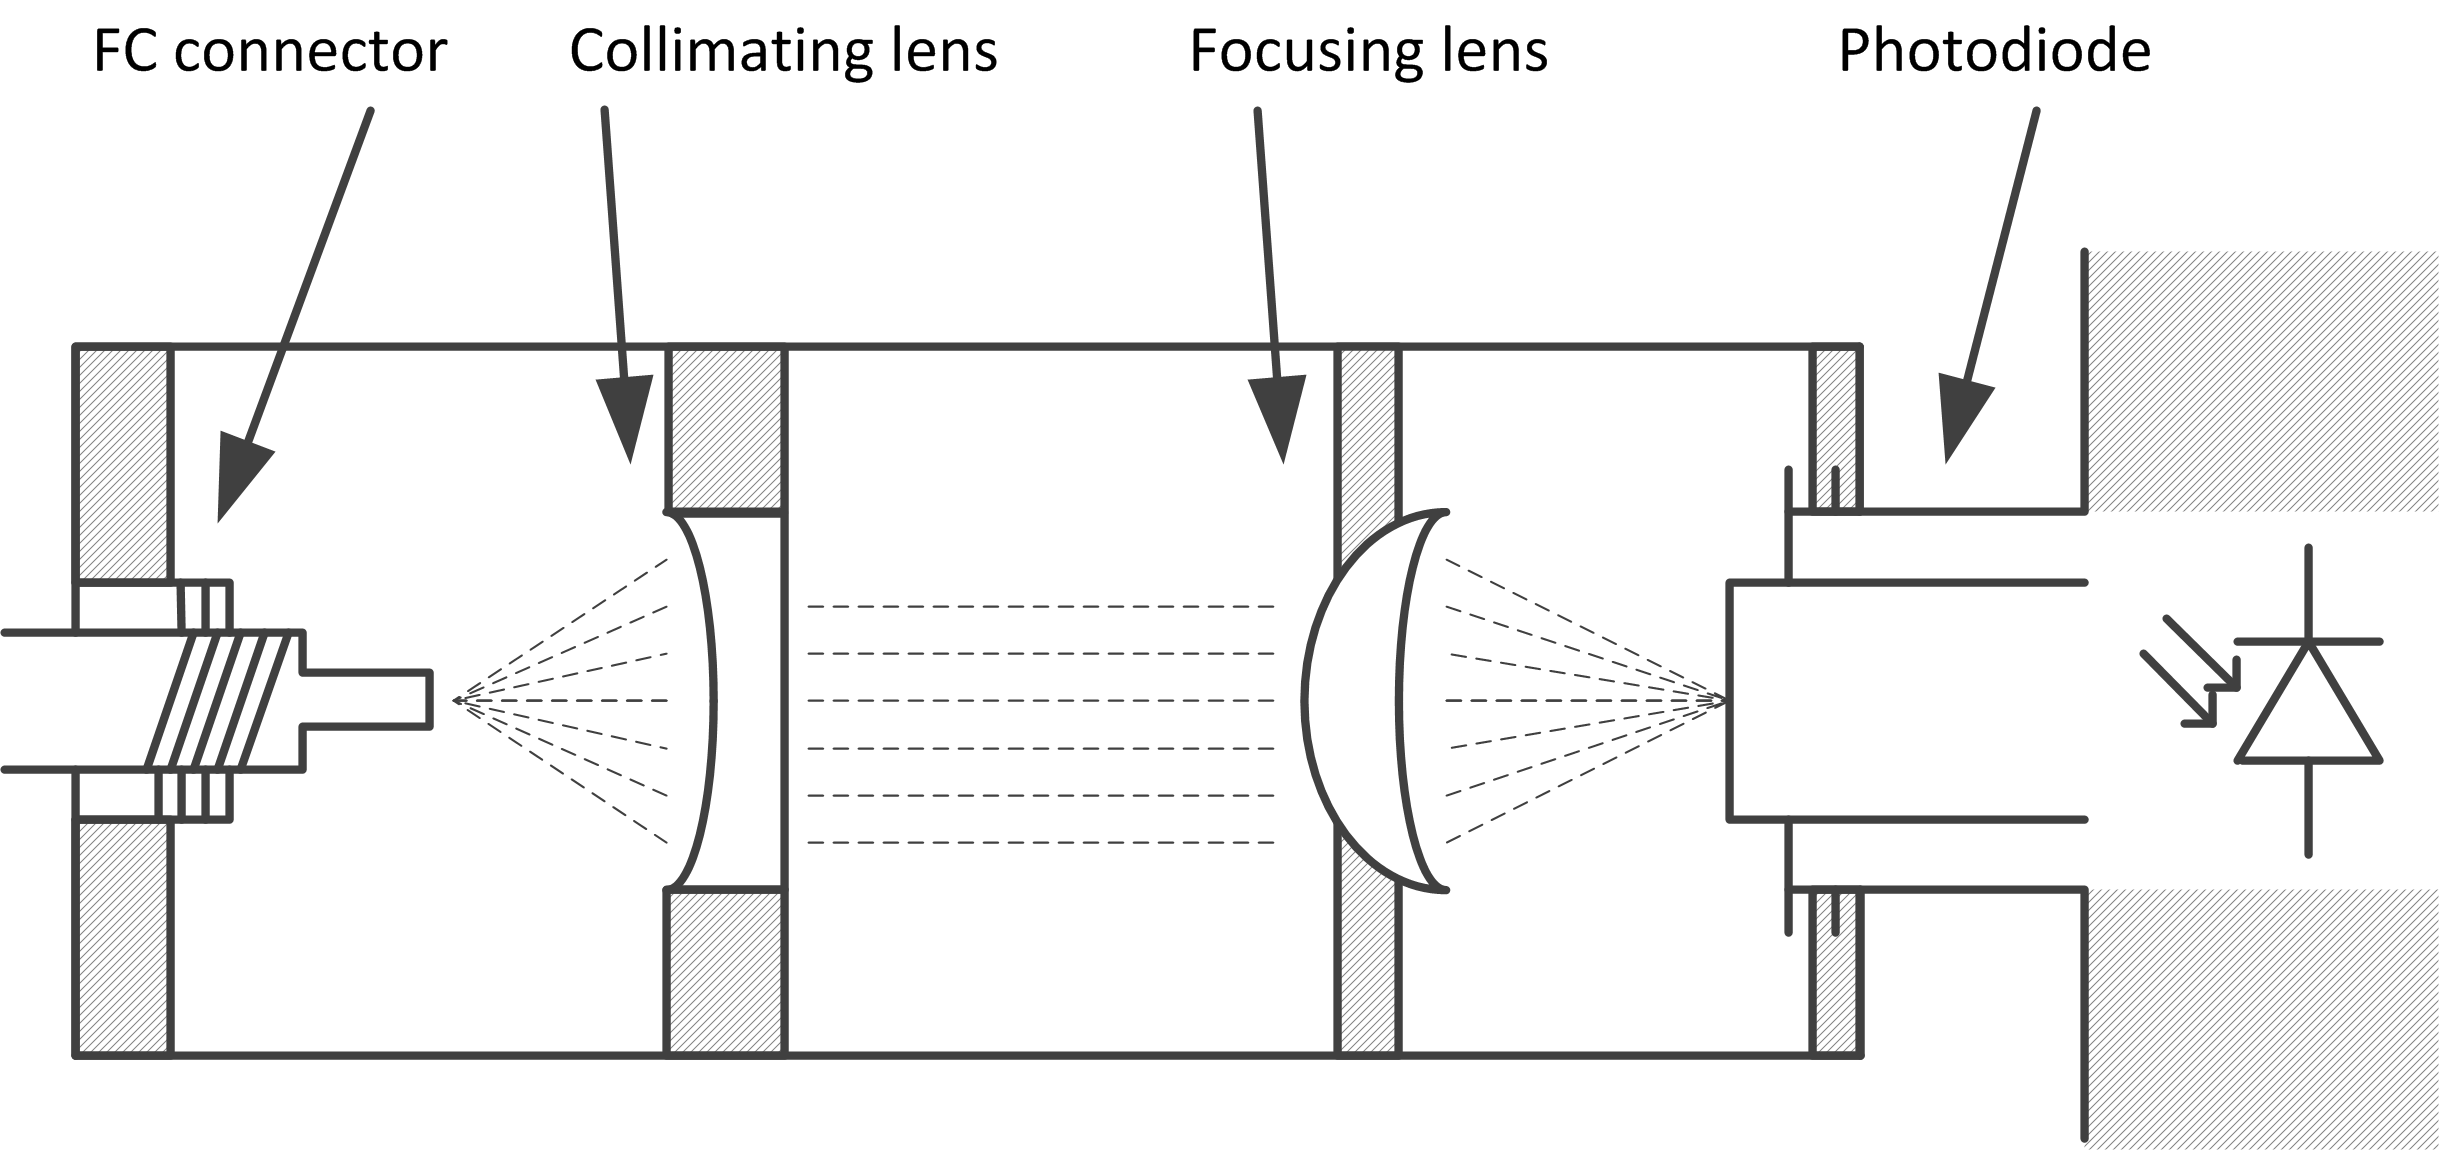
\includegraphics[width=0.9\textwidth]{apd_optics.png}
	\caption{APD optical setup}
	\label{fig:apd_optics}
\end{figure}
The photodetector was then connected to a constant-wave optical source. The additional optical components were then mechanically aligned, so that the received power became maximum, indicating good focusing and alignment. In this process, the same multi-mode fibres were used, as those used in actual anti-Stokes measurement scenario. \\

Photodetectors have a BNC connector at their output. This enables them to operate under a matched 50 \textOmega, or a high-impedance load. The transimpedance gain presented in Table \ref{table:photodetectors} is the gain achieved with the high-impedance load on the photodetector's output, as was the case in this laboratory setup. All the photodetectors' outputs were monitored by a DAQ device PXIe-5160 from National Instruments. The device is a 10-bit analogue-to-digital converter (abbr. ADC), its highest input frequency being \cite{datasheet:daq}
\begin{equation}
f_\textrm{max} = \SI{500}{\mega \hertz} \textrm{,}
\end{equation}
and the configured input impedance
\begin{equation}
Z_\textrm{in} = \SI{1}{\mega \ohm} \| \SI{15}{\pico \farad} \textrm{.}
\end{equation}
The sampling rate is
\begin{equation}
f_\textrm{S} = \SI{1.25}{\giga S / \second} \textrm{,}
\end{equation}
which ensures a faithful representation of the signal detected by the photodetector. Input voltage range was set to
\begin{equation}
V_\textrm{pk-pk} = \SI{50}{\milli \volt} \textrm{.}
\end{equation}
With a 10-bit ADC, the quantization step is
\begin{equation}
q \approx \SI{97.7}{\micro \volt} \textrm{.}
\end{equation}
This will prove sufficiently small when measuring the scattered signals to disregard the quantization noise of the ADC. The PXIe-5160 has an extension card form-factor, and is hosted by a National Instruments PXIe-1082 chassis. The system controller is also present in one of the chassis's slots. The extension card is declared to have a warm-up time of 15 minutes. Two channels, CH2 and CH3, of the DAQ device are used to monitor Stokes and anti-Stokes signals, respectively. On channel CH4 the output signal from an Analog Devices TMP36 calibrated temperature sensor is connected. This device is used to calibrate the temperature offset of the system, by determining the temperature at the beginning of the measurement fibre. The TMP36 is soldered onto a coaxial, and a USB cable in parallel. This enables power supply from the system controller's USB hub. The current temperature can be calculated from sensor's output as \cite{datasheet:tmp36}
\begin{equation}
T \, \textrm{[\textdegree C]} = \left( V \, \textrm{[mV]} - V_\textrm{n} \right) \cdot 0.1 \, \textrm{[\textdegree C / mV]} + 25 \, \textrm{\textdegree C}
\end{equation}
\begin{equation}
V_\textrm{n} = \SI{750}{\milli \volt} \textrm{.}
\end{equation} \\

To the CH1 channel of the DAQ card, a simple PIN photodiode, model PDA10CF-EC from Thorlabs, is connected. Its optical input is connected to the 1\% tap output from the laser. The signal is attenuated before reaching the photodetector by an attenuator that operates in the range
\begin{equation}
L_\textrm{att} \in [\SI{25}{\decibel}, \SI{30}{\decibel}] \textrm{.}
\end{equation}
The signal on channel CH1 is used for triggering data acquisition at the same time as the optical pulse is sent along the measurement fibre. Also, knowing the opto-electrical characteristics of the photodetector, one can use the measured peak value of the tap optical pulse to determine the peak optical power in the fibre. By monitoring the waveform acquired by the DAQ card, one can also observe the shape of the optical pulse. \\

The described laboratory setup enables simple replacement of photodiodes, testing of different fibre types and fibre combinations, and reconfiguration of the digital processing algorithm. Optical parts are connected by SC or FC connectors. These need to be thoroughly cleaned to ensure best performance. All the relevant optical parameters in the system can be monitored. 

% --------------------------------------

\setcounter{stranica}{\thepage}
\addtocounter{stranica}{1}

\end{document}